\documentclass[10pt,letterpaper,bibliography=totocnumbered]{scrartcl}

\usepackage[letterpaper,margin=1.2in]{geometry}
\usepackage{helvet}
\usepackage{graphicx}
\usepackage[hyphens]{url}
\usepackage{hyperref}
\usepackage[all]{hypcap} 
\usepackage{xcolor}
\usepackage{listings}
\usepackage[T1]{fontenc}
\usepackage{verbatim}

\lstset{
    basicstyle=\scriptsize,
    numbers=left,
    numberstyle=\scriptsize,
    stepnumber=1,
    numbersep=5pt,
    showspaces=false,
    showstringspaces=false,
    showtabs=false,
    frame=shadowbox,
    tabsize=4,
    captionpos=b,
    breaklines=true,
    breakatwhitespace=false,
    keywordstyle=\color{blue!70},
    commentstyle=\color{red!50!green!50!blue!50},
    rulesepcolor=\color{red!20!green!20!blue!20},
    numberbychapter=false,
    stringstyle=\ttfamily
}

\setcounter{tocdepth}{2}

\hypersetup{colorlinks=true,
breaklinks=true,
urlcolor=blue,
linkcolor=black
}

\begin{document}

\author{Mathew Chaney}
\title{Assignment 8}
\subtitle{Fall 2014\\ CS595 Web Science\\ Dr. Michael Nelson}
\maketitle
\newpage

\tableofcontents
% \listoffigures
\lstlistoflistings

\section{Question 1}

\subsection{Question}
\verbatiminput{q1/q1.txt}

\subsection{Answer}
Using Dr. Michael Nelson's Twitter account and the Twitter API \cite{api:twitter}, specifically the GET friends/list \cite{api:twitter_friendslist} request, all of Dr. Nelson's Twitter friends were obtained and saved to the file called {\tt friends}. This method also uses the API's paginating scheme: when there are a large number of results for a query, the API will send a cursor index to show that there are more results to process and that more requests are needed. The code to do this is in Listing \ref{listing:get_friends}. 

% \lstinputlisting[language=Python, caption={Getting the friends list}, label=listing:get_friends,linerange={38-57},firstnumber=38]{q1/get_friends.py}

\clearpage

To reduce the impact of high HTTP traffic, the Twitter API rate-limits most requests -- the one needed to obtain a user's friends list has a limit of fifteen message per fifteen minutes. Any requests received from a user or service that has reached the limit will be denied. To ensure no HTTP requests are sent after the limit has been reached the script will sleep until the limit resets. This is accomplished using Python's {\tt time} package \cite{py:time} and the methods shown in Listing \ref{listing:wait}.

% \lstinputlisting[language=Python, caption={Waiting for API request limit reset}, label=listing:wait,linerange={24-36},firstnumber=24]{q1/get_friends.py}

The {\tt get\_limit} method uses the API to find the number of available requests remaining for the GET friends/list method and also the time at which the limit will reset, received as seconds since the Unix epoch \cite{misc:stack_unixepoch}. This method, combined with the {\tt wait\_for\_reset} method, allowed the script to restart after an interruption and only require waiting for the appropriate amount of time. The sleep time was extended by 5 seconds to allow for a small buffer in case of mathematical errors.\\

The friends of Dr. Nelson's friends were then obtained with the same {\tt get\_friends} method from Listing \ref{listing:get_friends} and stored in a file called {\tt friend\_counts}, each on a single line preceeded by their friend count. All of these operations were controlled by a main method, which is shown in Listing \ref{listing:main}.

% \lstinputlisting[language=Python,caption={Main method}, label=listing:main, linerange={59-82},firstnumber=59]{q1/get_friends.py}

\clearpage

The {\tt friend\_counts} file was ordered in place with the Unix command in Listing \ref{listing:sort}. 

\begin{lstlisting}[language=Bash,caption={Sort command},label=listing:sort]
[mchaney@mchaney-l a5]$ cat friend_counts | sort -g -o friend_counts
\end{lstlisting}

This file was then processed by the R script shown in Listing \ref{listing:graph} to produce the graph in Figure \ref{fig:friend_graph}

% \lstinputlisting[language=R, caption={Graph Creation Script}, label=listing:graph]{q1/plot_friends.R}

\clearpage
The median, mean and standard deviation were all calculated, with the median, mean and median plus one standard deviation plotted as horizontal lines that intersect the data plot at their y-values. Only a single line was drawn for the standard deviation because the lower-end value was negative, and thus off the graph. 

% \begin{figure}[h!]
% \centering
% \fbox{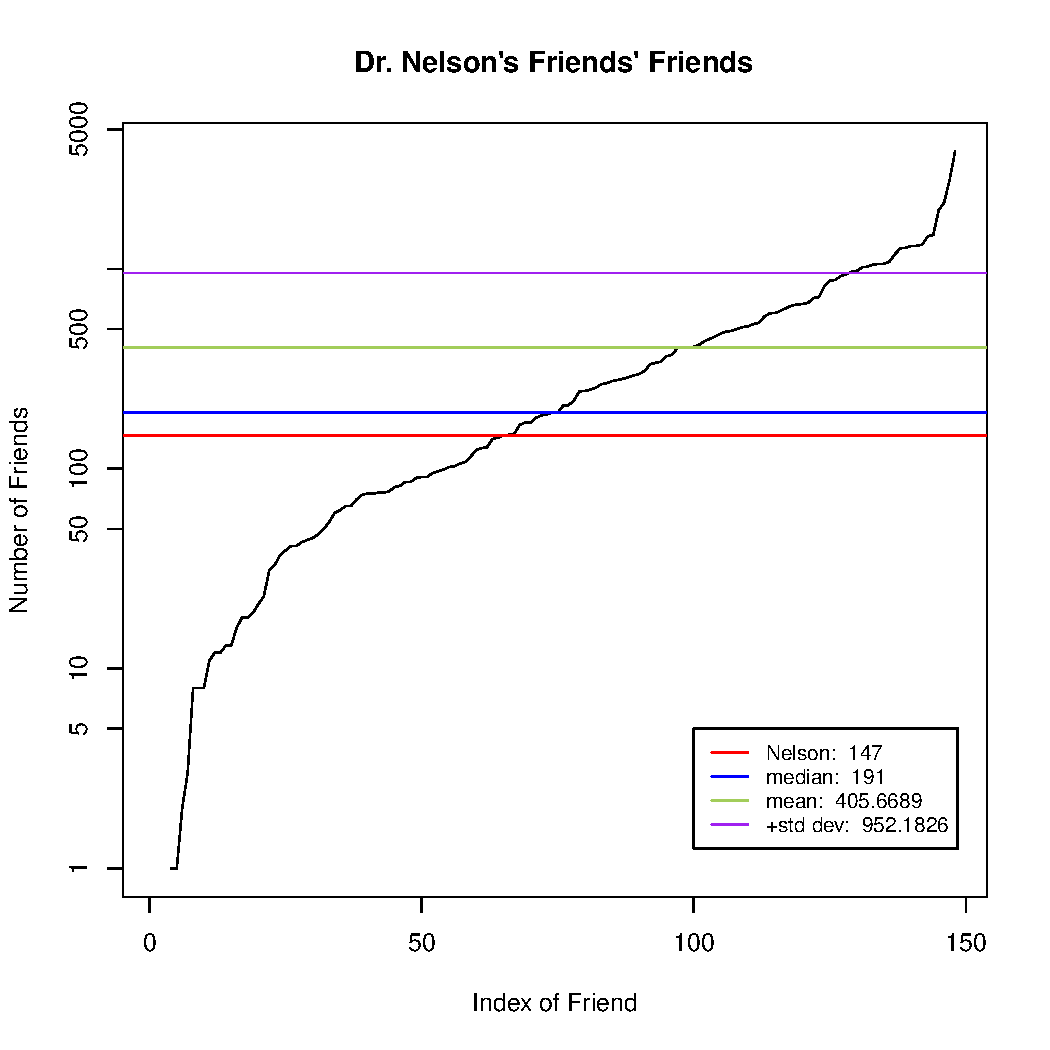
\includegraphics[scale=0.75]{q1/friend_plot.pdf}}
% \caption{The Friendship Graph}
% \label{fig:friend_graph}
% \end{figure}
\section{Question 2}

\subsection{Question}
\verbatiminput{q2/q2.txt}

\subsection{Answer}

% \lstinputlisting[language=Python, caption={all code used}, label=listing:all]{q1/recommendations.py}
\section{Question 3}

\subsection{Question}
Estimate the age of each of the 1000 URIs using the "Carbon Date" tool:\\

http://ws-dl.blogspot.com/2013/04/2013-04-19-carbon-dating-web.html\\

Note: you'll have better luck downloading and installing the tool 
rather than using the web service (which will run slowly and likely
be unreliable).\\

For URIs that have > 0 Mementos and an estimated creation date,
create a graph with age (in days) on one axis and number of mementos
on the other.\\

\subsection{Resources}
\begin{itemize}
\item None: yet
\end{itemize}

\subsection{Answer}

\section{Question 4}

\subsection{Question}
\verbatiminput{q4/q4.txt}

\subsection{Answer}

With the code in Listing \ref{listing:scaledownmain}, multidimensional scaling (MDS) was used to create a two-dimensional visualization of the blog distance graph.

\lstinputlisting[language=Python, caption={main for scaledown}, label=listing:scaledownmain,linerange={301-302},firstnumber=301]{q2/clusters.py}

This main code calls the scaledown function, which is shown in Listing \ref{listing:scaledownfunc}. The algorithm continues until the error factor stops decreasing, as shown in the output in Appendix A, Listing \ref{scaledown}. 

\lstinputlisting[language=Python, caption={scaledown function}, label=listing:scaledownfunc,linerange={224-272},firstnumber=224]{q2/clusters.py}

The scaledown function returns the coordinates for each of the blogs in 2D space. This data was then used with the {\tt draw2d} function in Listing \ref{listing:draw2d}, which produced the two-dimensional visualation created from the MDS algorithm, as shown in Figure \ref{fig:blogs2d}.

\lstinputlisting[language=Python, caption={draw2d function}, label=listing:draw2d,linerange={274-281},firstnumber=274]{q2/clusters.py}

\begin{figure}[h!]
\centering
\fbox{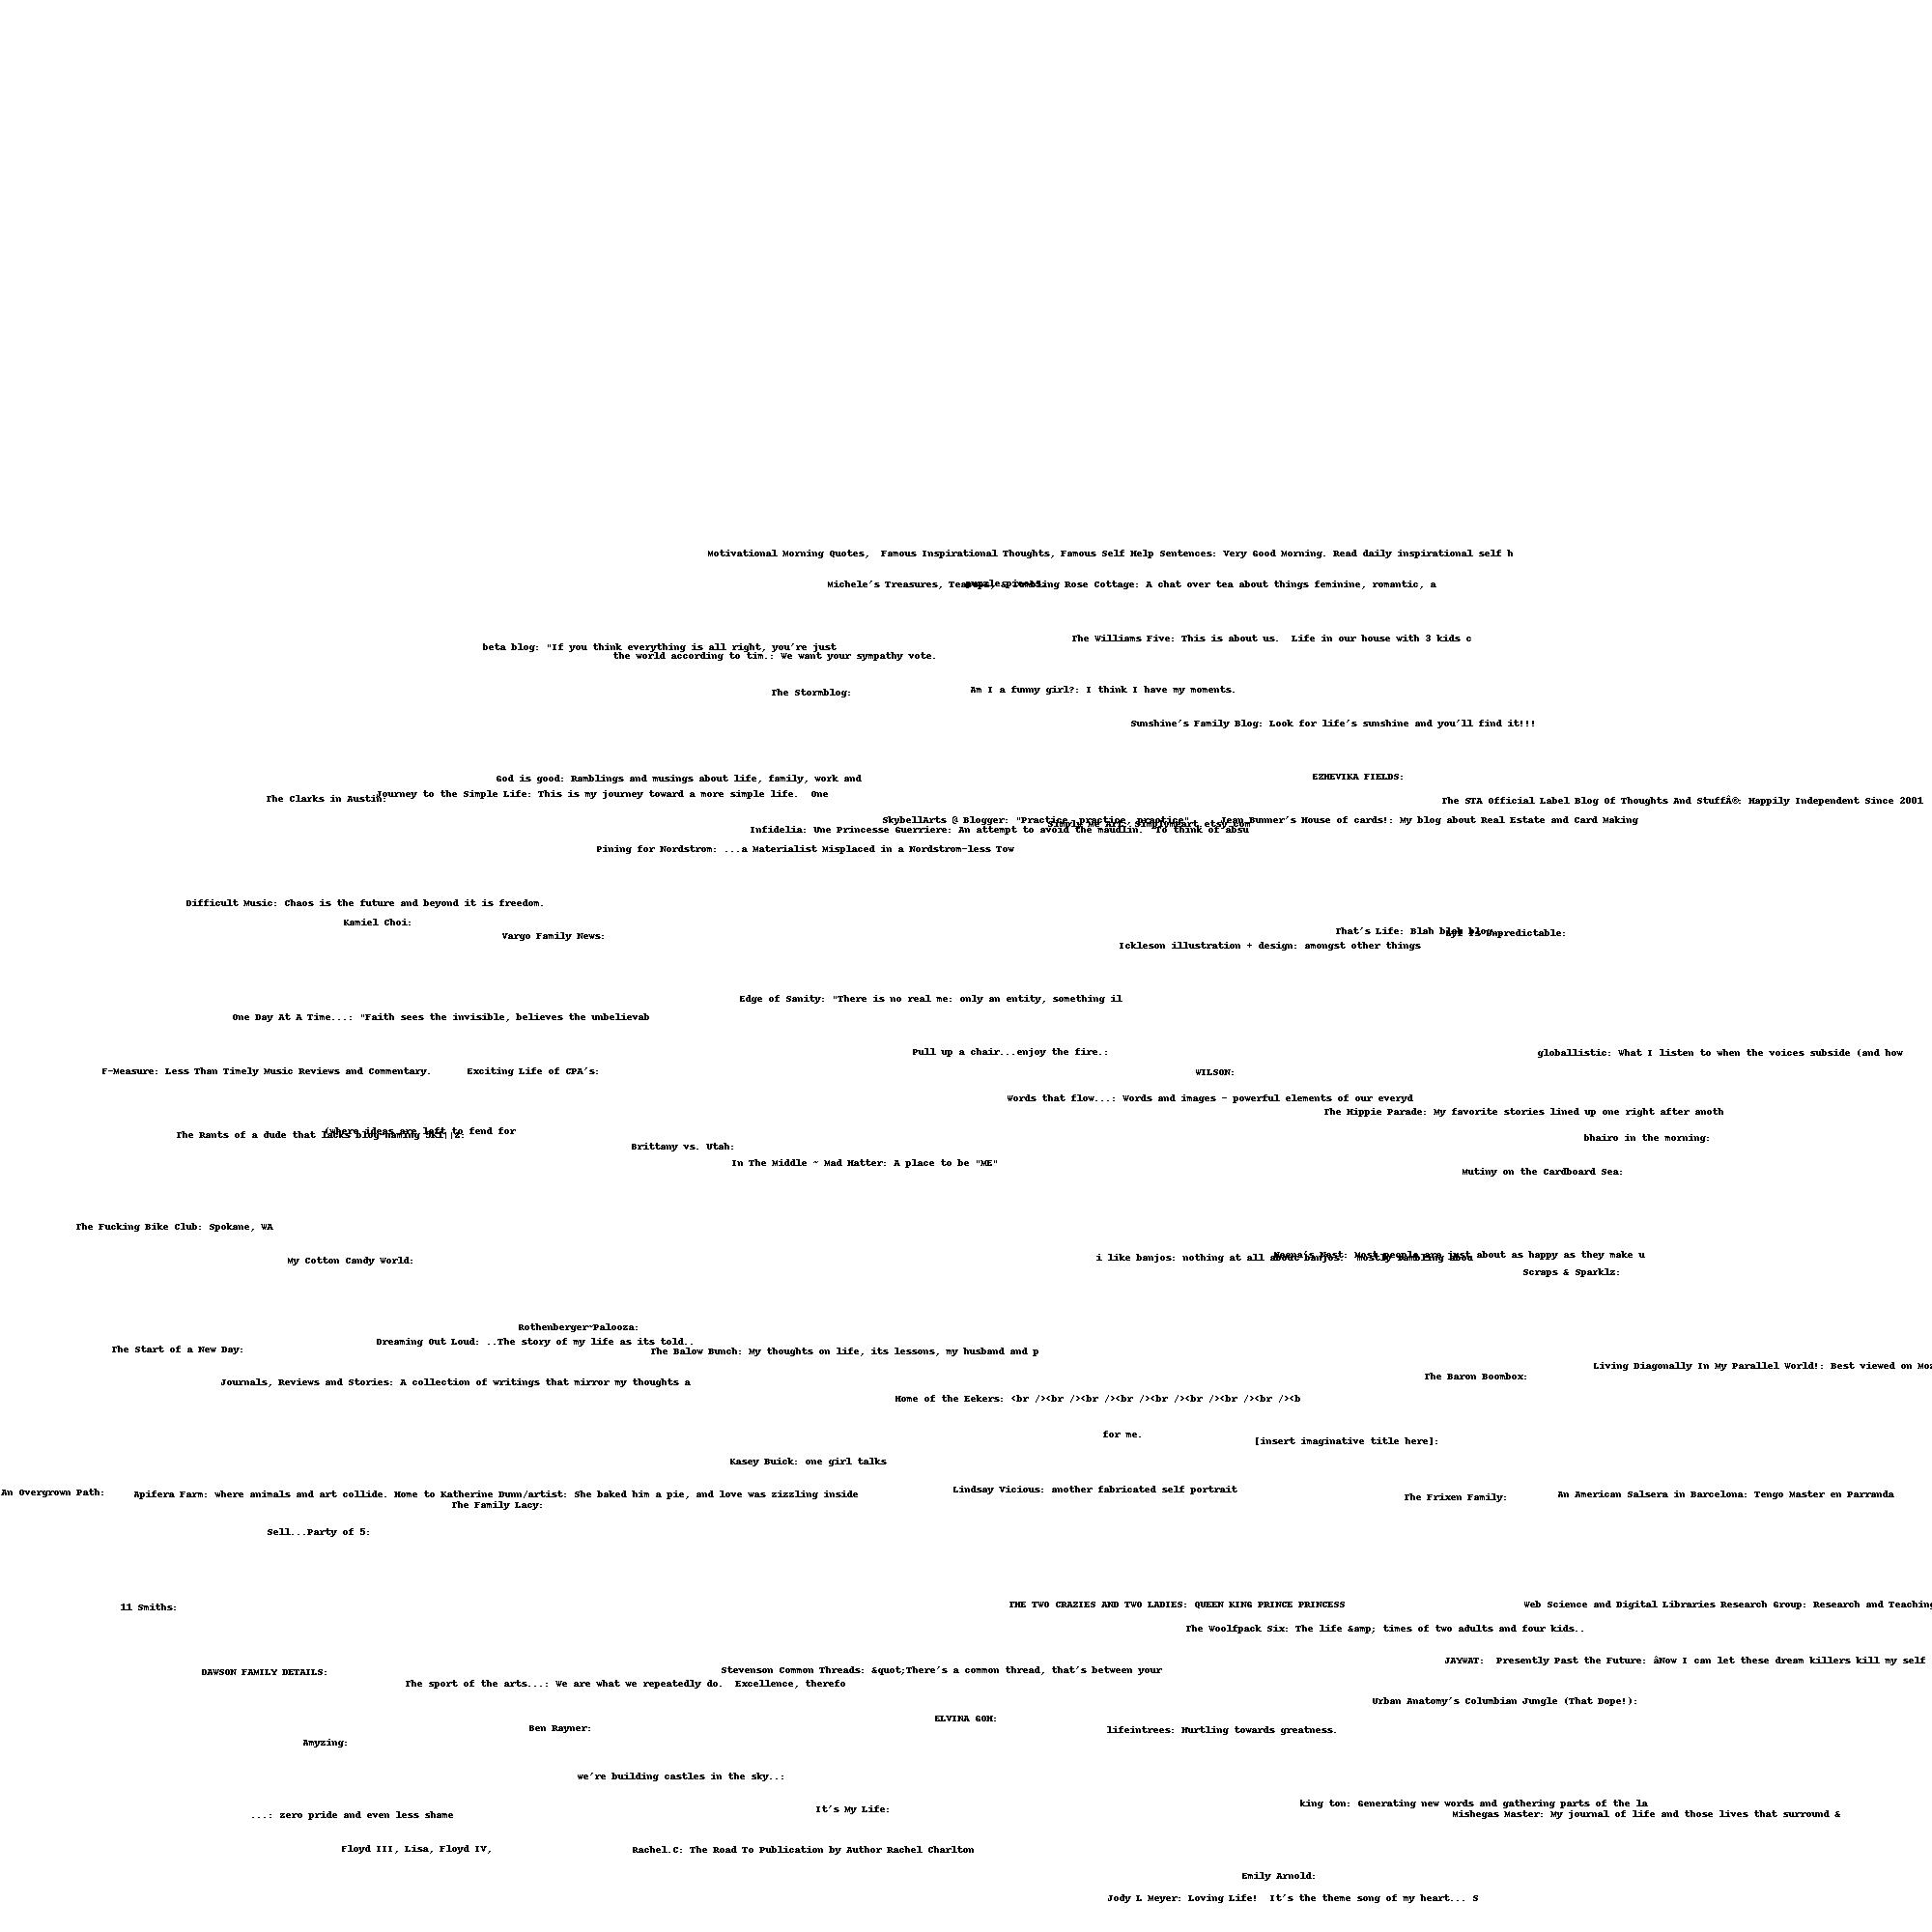
\includegraphics[trim=0 0 0 500, clip, scale=0.2]{q4/blogs2d.jpg}}
\caption{MDS 2d visualization}
\label{fig:blogs2d}
\end{figure}
\section{Question 5}

\subsection{Question}
\verbatiminput{q5/q5.txt}

\subsection{Answer}

To answer this question, {\tt matrix.py} was modified to add the capability to calculate {\it Term Frequency Inverse Document Frequency (TF/IDF)}. The added functions for computing TF/IDF are found in Listing \ref{listing:tfidf}. These functions use the master word count dictionary ({\tt wordcounts}) and each blog's individual word count ({\tt wc}) for each of the words in the {\tt wordlist} from Question 1/2 to compute the TF/IDF value for each word in the word list. 

\lstinputlisting[language=Python, caption={use of tfidf function},label=listing:tfidfmain,linerange={116-117},firstnumber=116]{matrix.py}

\lstinputlisting[language=Python, caption={writing the data}, label=listing:matrix:writedata, linerange={79-93}, firstnumber=79]{matrix.py}

\lstinputlisting[language=Python, caption={tf idf functions},label=listing:tfidf,linerange={40-48},firstnumber=40]{matrix.py}

The same clustering was applied to the TF/IDF result matrix as was done in Question 2 and both images are displayed in Figures \ref{fig:plain} and \ref{fig:tfidf}.

There are a many pairs that were found to be similar in both clusterings. For example, in both dendrograms, the {\it Web Science and Digitial Libraries Research Group} blog is most similar to the {\it ...: zero pride and even less shame} blog, the {\it DJ DHANIEL FAN AND PRODUCER} and {\it The Baron Boombox}, among a few others. In spite of this, the larger groupings do not appear very similar between the two clustings.

When examining the clusters on a larger scale, it seems that the TF/IDF dendrogram clustered blogs are subjectively more alike better than the raw count version did. Looking toward the bottom of the TF/IDF clustering image, one will notice a grouping of blogs that seem closely related to music: {\it F-Measure: Less Than timely Music Reviews and Commentary.}, {\it Urban Anatomy's Columbian Jungle (That Dope!)} which seems to be a melding of fashion and music commentary, {\it Ezhevika Fields} a blog where info and preview samples of ``lost album samples of the past'' can be found, whereas these blogs are not all grouped together in the raw count version. It seems that using TF/IDF as a basis for document comparison gives much more context than a raw term count (which doesn't take into consideration the rest of the document in which each word resides).

There is another cluster in the TF/IDF driven image that seems to contain family related blogs, with blogs like {\it Am I a funny girl?: I think I have my moments}, {\it The Frixen Family}, {\it When Two Hearts Become One: A wife, a mom, a daughter, a sibling.} and {\it The Clarks in Austin} all being related to a particular family and their everyday lives. Some of these blogs are close to each other in the raw count version, but they are not separated into their own distinct groups.

When looking at the overall structure of each dendrogram, it becomes apparent that there are more individual clusters grouped together in the TF/IDF version than are present in the raw count image, where there seems to be few small clusters and one mega-cluster in the center. This suggests that the TF/IDF algorithm is better at defining discrete subgroups within a larger context than a simple raw count driven dendrogram will produce.

\begin{figure}[h!]
\centering
\fbox{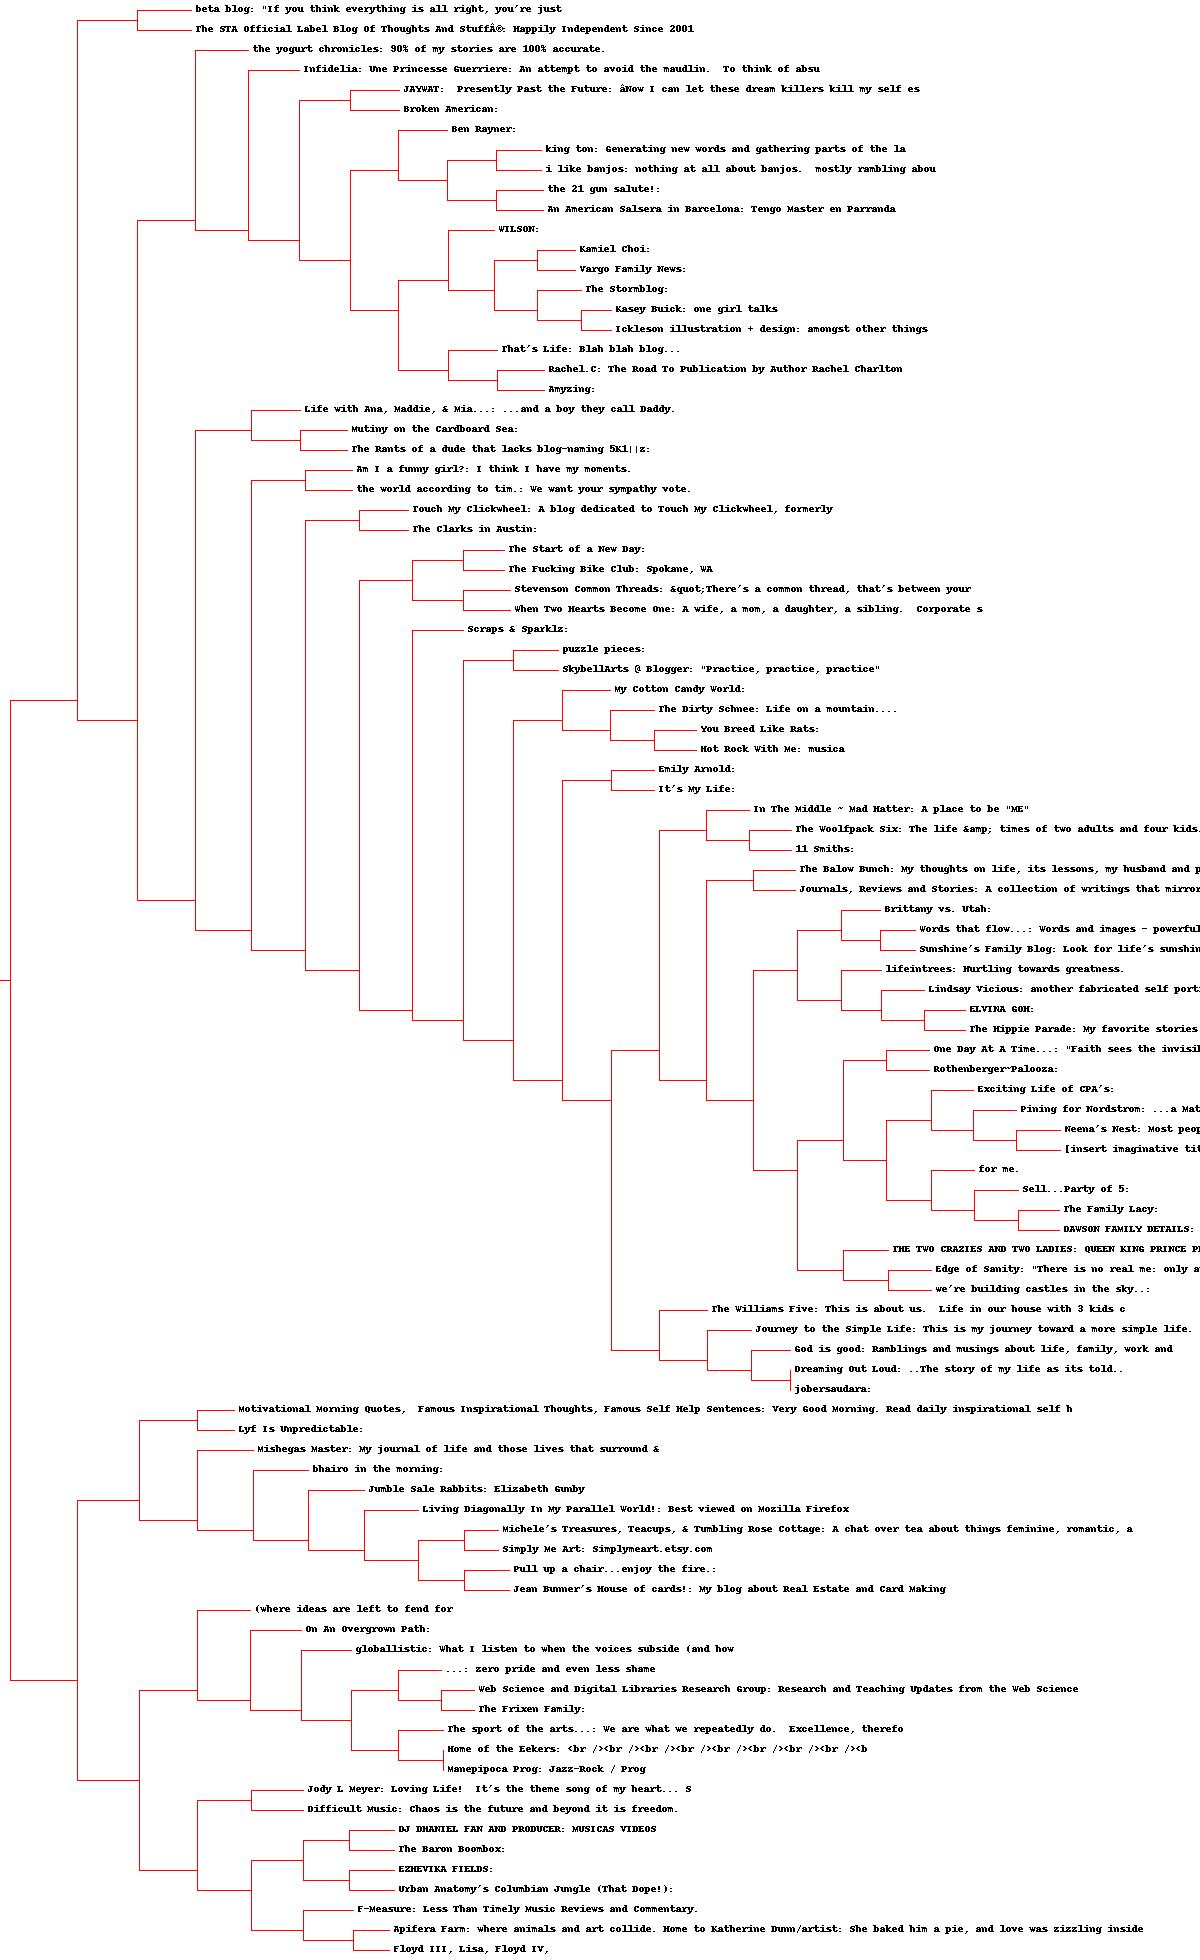
\includegraphics[scale=0.3]{q2/blogclust.jpg}}
\caption{plain count dendrogram}
\label{fig:plain}
\end{figure}

\begin{figure}[h!]
\centering
\fbox{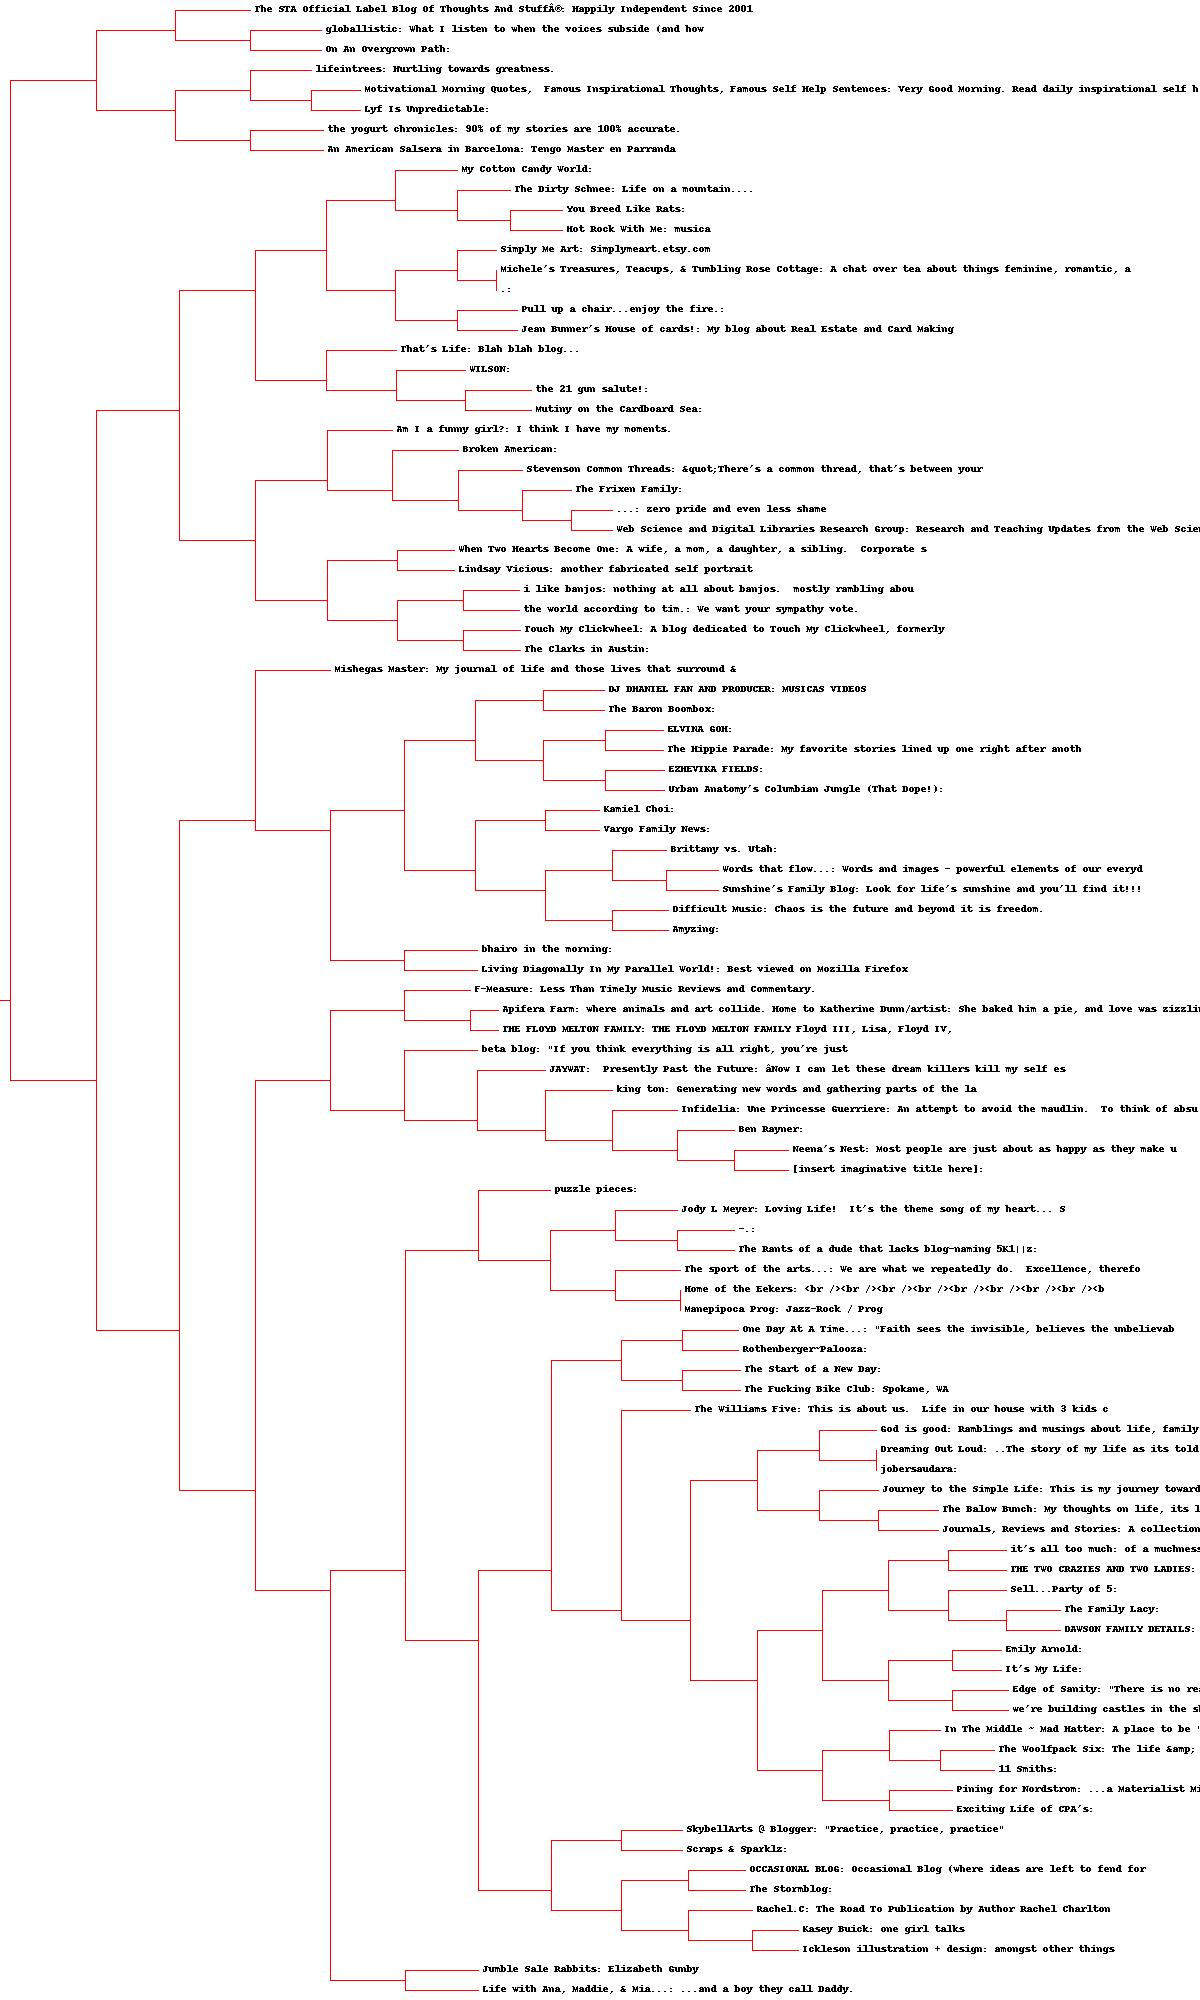
\includegraphics[scale=0.3]{q5/blogclust.jpg}}
\caption{TF/IDF driven dendrogram}
\label{fig:tfidf}
\end{figure}
\section{Appendix A} \label{appdx}

\lstinputlisting[language=Python, caption={get\_uris.py}, label=listing:get_uris]{q1/get_uris.py}

\clearpage

\lstinputlisting[language=Python, caption={matrix.py}, label=listing:matrix]{matrix.py}

\clearpage

\lstinputlisting[language=Python, caption={clusters.py}, label=listing:clusters]{clusters.py}

\clearpage

\lstinputlisting[language=Bash, caption={scaledown output}, label=scaledown]{q4/scaledown.txt}

\bibliography{report}
\bibliographystyle{unsrt}

\end{document}
